\chapter{Mise en place d'une solution \acentreon{}}
\label{section:centreon}

\section{La solution \acentreon}

\paragraph{}
\acentreon{} est une plateforme open source de supervision, c'est-à-dire de surveillance du bon fonctionnement d'une infrastructure système.

\paragraph{Principe de la supervision}
De façon classique, on surveille toutes les informations relatives au matériel (température, pannes\ldots) et au système (charge serveur, utilisation de la mémoire et du processeur\ldots) des serveurs d'un parc.
Généralement, on supervise également tous les services applicatifs (serveurs web, serveurs FTP, serveurs de base de données\ldots) qui y sont hébergées.

Ainsi, les administrateurs système peuvent savoir en temps réel quels sont les services et les machines qui sont fonctionnels ou hors-service.
Très souvent, des alertes leurs sont envoyées pour les prévenir d'une rupture de service.
Ces alertes peuvent prendre la forme d'e-mails mais aussi de SMS ou de messages envoyés par messagerie instantanée.

\paragraph{\anagios}
La solution \acentreon{} repose sur \anagios{} pour effectuer toutes les opérations de surveillance, de reporting et de d'alerte.
Par défaut, \anagios{} propose un certain nombre de possibilités que ce soit pour superviser les ressources des serveurs, les services actifs en consultant un port\footnote{Correspondant à la couche de transport du modèle OSI, la notion de port logiciel permet, sur un ordinateur donné, de distinguer différents interlocuteurs. Ces interlocuteurs sont des programmes informatiques qui, selon les cas, écoutent ou émettent des informations sur ces ports. Un port est distingué par son numéro.~\cite{port}} donné ou en interrogeant les machines via le protocole SNMP\footnote{SNMP (pour \etranger{Simple Network Management Protocol}) est un protocole de communication qui permet aux administrateurs réseau de gérer les équipements du réseau, de superviser et de diagnostiquer des problèmes réseaux et matériels à distance.~\cite{snmp}}.

Les possibilités de supervision sont infinies car \anagios{} est doté d'un système de plugins très efficace.
En effet, ces plugins sont de simples programmes exécutables via la ligne de commande, auxquels on passe en paramètre des options de configuration et qui retournent un entier.
On peut donc les développer dans n'importe quel langage de programmation.
C'est la valeur du code retour qui précise si le test effectué par le plugin est passé ou non :

\begin{description}
	\item[0 OK] le test est passé ;
	\item[1 WARNING] le seuil d'alerte est dépassé ;
	\item[2 CRITICAL] le service a un problème ;
	\item[3 UNKNOWN] il est impossible de connaître l'état du service.
\end{description}

Ces différents niveaux, en plus de permettre le déclenchement d'alertes, sont facilement distinguables sur l'interface web de \anagios{} via un code couleur (\cffigure{centreon:nagios}).

Enfin, il est possible de lancer des actions de surveillance à distance via le protocole NRPE (\etranger{Nagios Remote Plugin Executor}).
En effet, celui-ci permet de lancer n'importe quel plugin \anagios{}, si celui-ci est bien installé sur la machine interrogée.
Les informations transitent entre le serveur \anagios{} et les machines surveillées via un tunnel SSL\footnote{SSL (pour \etranger{Secure Sockets Layer}) est un protocole de sécurisation des échanges sur Internet.~\cite{tls}} sécurisé.

\begin{figure}
	\centering
	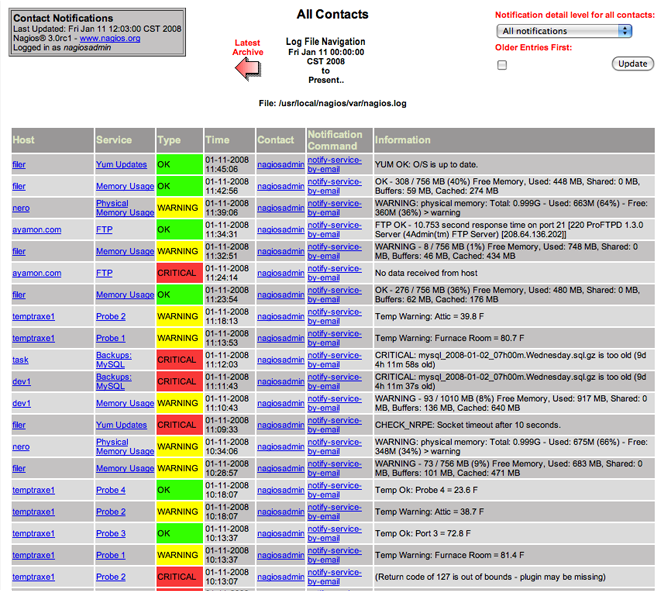
\includegraphics[width=12cm]{centreon/nagios-notifications}
	\caption{Historique des notifications sur Nagios}
	\label{figure:centreon:nagios}
\end{figure}

\paragraph{\acentreon}
Le principal avantage de ce complément à \anagios{} est de fournir une interface graphique web efficace, claire et plus simple à appréhender (\cffigure{centreon:centreon}).

Il ajoute entre autres une gestion fine des utilisateurs, des plugins \anagios{} supplémentaires, des représentations graphiques élaborées, des possibilités d'architecture distribuée, etc.

\begin{figure}
	\centering
	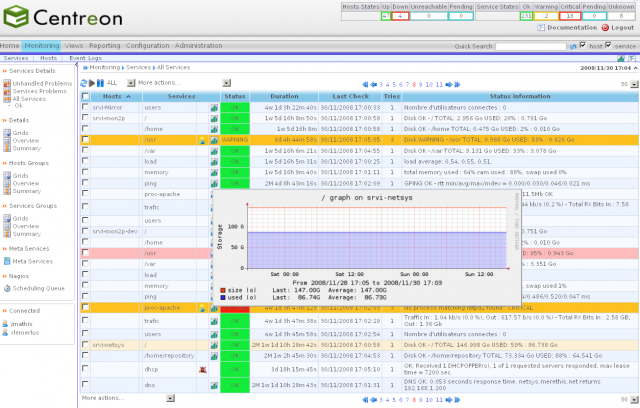
\includegraphics[width=12cm]{centreon/centreon-status}
	\caption{État en temps réel des services sur \acentreon{}}
	\label{figure:centreon:centreon}
\end{figure}


\section{Contexte de la mission}

\paragraph{}
Le client de \asmile{} pour cette mission était \adacast.
C'est une relativement jeune startup présente en France et aux États-Unis.
Son concept est de fournir une plateforme de diffusion multimédia à la demande, en live ou non, performante et simple à utiliser.
Ainsi, ses clients fournissent leurs flux audio ou vidéo et c'est \adacast{} qui se charge de les transformer dans le bon format et les diffuser tout en supportant les éventuels pics d'audience.
\adacast{} propose également différentes façon de monétiser les diffusions, que ce soit par la publicité, par un paiement à la vue ou au forfait.

\paragraph{}
Dans ce contexte, \adacast{} souhaite s'équiper d'une solution de supervision pour surveiller en temps réel son parc de serveurs.
En effet, jusqu'ici, les vérifications de disponibilité de ses services étaient relativement primaires alors que son offre, son nombre de clients et ses enjeux deviennent de plus en plus importants.
Toute rupture de service devient vite critique et doit être prise en charge dans les plus brefs délais.
Il s'agit aussi pour \adacast{} de faire preuve de professionnalisme envers ses clients en dépannant les problèmes avant de recevoir tout coup de fil de plainte.

\paragraph{}
Chez \asmile{}, \asegir{} est le spécialiste de la solution de supervision \acentreon{}.
Je l'ai donc suivi lors de son intervention chez \adacast{} pour apprendre à maîtriser cette technologie.
Nous avons travaillé ensemble la première journée durant laquelle il m'a formé, et j'ai pu terminer la mission seul le lendemain.
\asegir{} est ensuite intervenu à nouveau pour fournir une documentation et former les utilisateurs.


\section{Notre démarche}

\paragraph{}
Pour réduire les coûts et limiter le temps d'intervention, \adacast{} n'a commandé que l'installation de la solution \acentreon{} et la supervision de deux serveurs.
La supervision des autres serveurs serait alors effectuée par ses ressources internes.

\paragraph{}
Pour installer la plateforme \acentreon{}, nous avons demandé à notre interlocuteur de nous fournir un serveur indépendant.
En effet, il est important que la solution de supervision soit sur un serveur qui soit indépendant des serveurs à surveiller.
L'intérêt est à la fois de séparer les services et de ne pas être soumis aux même pannes que ce qui doit être supervisé.

Le client a choisi de commander un serveur à bas coût -- de l'ordre de 20\euro~HT par mois -- chez un hébergeur externe.
Une telle configuration minimaliste est suffisante pour le besoin car peu d'utilisateurs vont consulter la plateforme \acentreon{} et le trafic relatif à l'échange de données de surveillance est limité.

\asegir{} m'a alors montré comment installer \acentreon{} sur un système \alinux{} Ubuntu Server.

\paragraph{}
Nous sommes ensuite passés à la partie la plus intéressante de l'intervention, c'est-à-dire la configuration de la solution en fonction des besoins du client.
Pour cela, des démons NRPE ont été installés sur chaque serveur à superviser.
Nous avons alors mis en place un certain nombre de plugins pour couvrir le périmètre attendu, qui inclut entre autres :

\begin{itemize}
	\item la surveillance des ressources des machines (consommation processeur et mémoire, charge serveur, espace disque disponible) ;
	\item le fonctionnement du RAID matériel ;
	\item la surveillance de la disponibilité de ses services (HTTP, MySQL, FTP, SSH, etc.) ;
	\item la surveillance des métriques relatives à l'utilisation de leur base de données MySQL.
\end{itemize}

\paragraph{}
Enfin, une vue d'ensemble de l'architecture mise en place est illustrée en \reffigure{centreon:archi}.

\begin{figure}
	\centering
	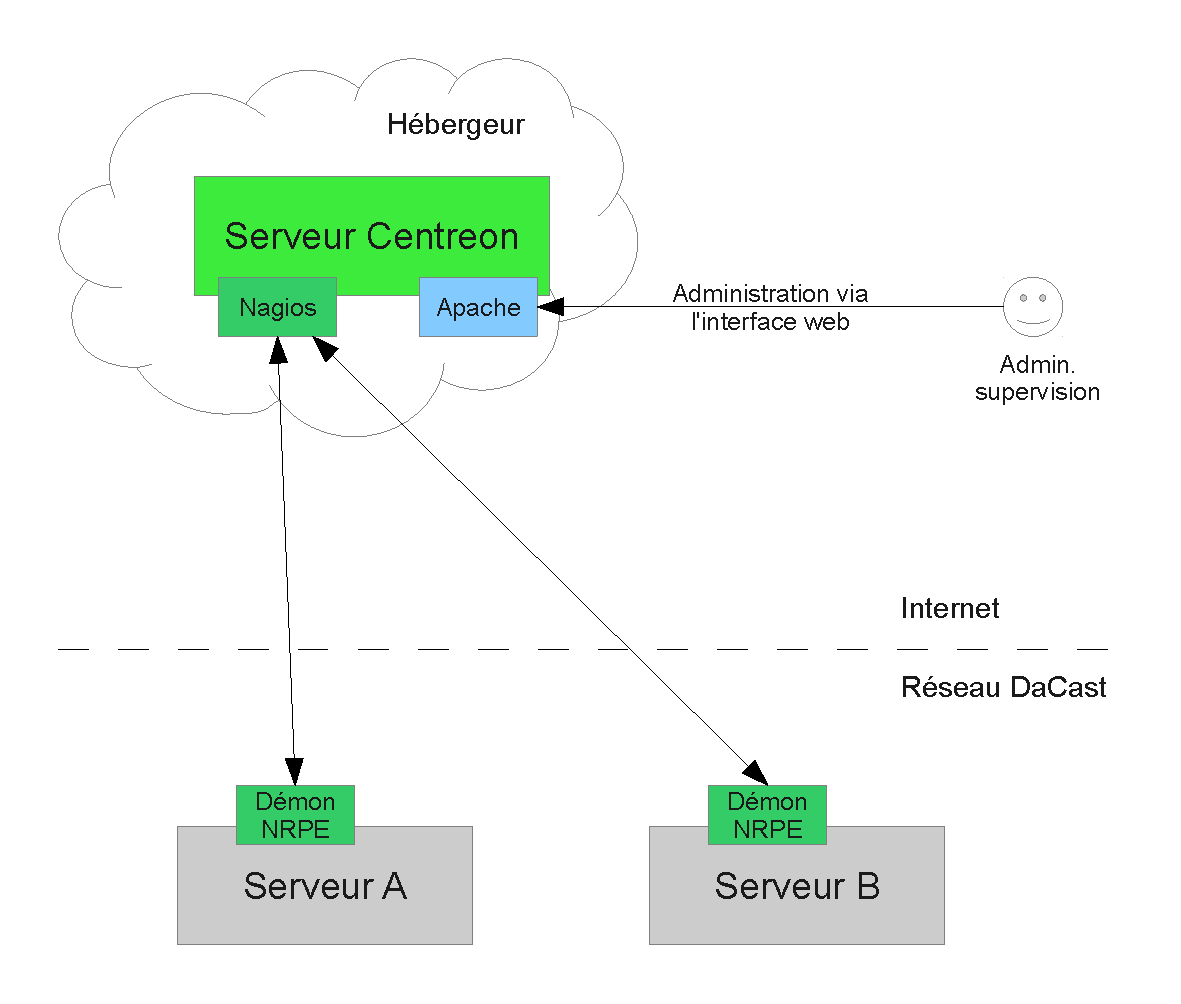
\includegraphics[width=12cm]{centreon/archi}
	\caption{Architecture de supervision mise en place chez \adacast{}}
	\label{figure:centreon:archi}
\end{figure}

